\documentclass[14pt]{matmex-diploma-custom}

\usepackage{graphicx}
\usepackage{subfigure}

\begin{document}
\filltitle{ru}{
  chair = {Программная инженерия},
  title = {Система сбора и анализа показателей жизнедеятельности на основе данных с мобильных устройств},
  type = {bachelor},
  position = {студента},
  group = 471,
  author = {Байгельдин Александр Юрьевич},
  supervisorPosition = {к.\,ф.-м.\,н., доцент},
  supervisor = {Романовский К.\,Ю.},
  reviewerPosition = {Зам. ген. директора ООО ``ПитерСофтвареХаус''},
  reviewer = {Хитров Д.\,В.},
  year = {2018}
}
\filltitle{en}{
  chair = {Software Engineering},
  title = {System for collection and analysis of vital signs based on data from mobile devices},
  author = {Aleksandr Baigeldin},
  supervisorPosition = {assistant professor},
  supervisor = {Konstantin Romanovsky},
  reviewerPosition = {Deputy director general of ``PiterSoftwareHouse'' Ltd.},
  reviewer = {Denis Khitrov},
  university = {Saint Petersburg State University},
}
\maketitle
\tableofcontents

\section*{Введение}
Стресс --- это совокупность неспецифических (т.е. независимых от типа стрессора)
адаптационных реакций организма на воздействие различных факторов (физических
или психологических), нарушающих его гомеостаз (стабильное, равновесное
состояние) \cite{book:stress_of_life}. В современной медицине принято разделять
понятие положительного стресса (эустресса) и отрицательного стресса (дистресса)
\cite{article:eustress_distress}. В результате положительного стресса повышается
функциональный резерв организма, происходит его адаптация к стрессовому фактору
и ликвидация самого стресса. Однако, когда организм постоянно подвергается
стрессу или же стрессор слишком сильный, защитные силы организма истощаются и он
становится не в состоянии самостоятельно справиться со стрессом. От такого
стресса страдает иммунная система, он подрывает здоровье человека и способствует
развитию тяжелых заболеваний, таких как депрессивное расстройство, диабет и даже
рак \cite{article:stress_and_illness}. В связи с этим, получили широкое развитие
различные методы управления стрессом, которые помогают предупреждать его
отрицательное воздействие. Однако, зачастую человек не замечает или не осознает
того, что подвергается воздействию стресса. Поэтому перспективной областью
исследования является автоматическое отслеживание стресса в повседневной жизни в
реальном времени.

Поскольку основное воздействие стресс оказывает на нервную и эндокринную системы
организма, то для его определения логичным является поиск соответствующих
шаблонов в работе этих систем. Например, анализ крови может выявить повышенное
содержание кортизола (глюкортикоидного ``гормона стресса'') в крови. Однако,
инвазивные методы не подходят для непрерывного отслеживания стресса. В связи с
этим, особый интерес вызывает реакция нервной системы организма на стресс, а
если точнее, то реакция симпатического отдела автономной нервной системы,
который отвечает за мобилизацию сил организма в экстренных ситуациях.
Симпатическая нервная система оказывает влияние на частоту сердцебиения и
дыхания, кровяное давление, электрическую активность кожи и другие показатели.
Поэтому диапазон медицинских сенсоров, с помощью которых можно в той или иной
мере определять стресс, довольно обширен: пульсометры, тонометры, GSR сенсоры, и
т.д. Тем не менее, наиболее перспективным типом сенсоров для задачи отслеживания
стресса в реальном времени являются именно пульсометры, т.к. несмотря на
небольшую цену, они обладают необходимой мобильностью и предоставляют
возможность высчитывать один из самых важных показателей активности
симпатической нервной системы --- вариабельность сердечного ритма
\cite{article:hrv_stress}.

Однако, симпатическая нервная система реагирует даже на небольшие стрессоры,
которые нет смысла учитывать в статистике, но которые при этом оказывают влияние
на вариабельность сердечного ритма. Например, даже при медленной ходьбе
вариабельность сердечного ритма отличается от сидячего положения
\cite{article:hrv_reliability}, хотя нельзя назвать ходьбу стрессом в
отрицательном смысле. Поэтому учет физической активности (например, на основе
данных с акселерометра) является хорошим способом отфильтровать ложные
срабатывания отслеживающей стресс системы. Для комбинации показателей физической
активности и показателей активности симпатической нервной системы при
определении стресса можно применить популярное на сегодняшний день в медицине
машинное обучение.

Таким образом, для задачи автоматического отслеживания стресса в реальном
времени требуется система, которая бы определяла стресс на основе данных с
пульсометра и акселерометра и обладала бы достаточной мобильностью для того,
чтобы применять ее в повседневной жизни.
	
\section{Постановка задачи}
Целью данной работы является создание прототипа мобильного приложения,
отслеживающего человеческий стресс в реальном времени, определяя его на основе
данных полученных с акселерометра мобильного телефона и внешнего пульсометра,
применяя для этого машинное обучение.

Для достижения этой цели были поставлены следующие задачи:

\begin{itemize}
\item Исследовать природу человеческого стресса и изучить публикации на тему
  определения стресса на основе медицинских данных.
\item Спроектировать архитектуру приложения и его взаимодействия с медицинскими
  сенсорами и моделью машинного обучения.
\item Реализовать мобильное приложение и добавить в него функциональность для
  сбора данных.
\item Собрать данные для обучения модели, обучить модель и оценить ее
  эффективность.
\end{itemize}

\section{Обзор}
\subsection{Физиология стресса}
Каким бы не был стресс, эмоциональным или физическим, организм всегда реагирует
на него одинаково. Именно поэтому стресс определяется как неспецифическая
реакция организма. Это значит, что вне зависимости от того, положительное ли
событие произошло (например, победа в соревновании) или отрицательное (например,
получение физической травмы), в организме активируются одни и те же механизмы.
Разница в положительном и отрицательном стрессе заключается только в том, смог
ли организм с ним справиться до того, как истощились его ресурсы, т.е. чем чаще
организм подвергается конкретному стрессору и чем он продолжительнее и
интенсивнее, тем больше вероятность, что данный стрессор отрицательно влияет на
организм.

Любой стресс начинается со стадии тревоги, которая не зависит от типа стрессора,
может длиться от нескольких часов до нескольких суток и всегда проявляется
одинаково (через активацию соответствующих систем организма). Затем идет стадия
сопротивления, в течение которой организм пытается адаптироваться к специфичному
типу стрессора, повышая свою устойчивость к его воздействию, и приводя в норму
системы, которые были активированы на предыдущей стадии. Далее может идти либо
стабилизация, либо (если стресс был слишком интенсивный или продолжительный)
стадия истощения. Этот процесс, состоящий из трех стадий (тревоги, сопротивления
и истощения), получил название общего адаптационного синдрома.

Поэтому очень важно предупреждать стресс еще на стадии тревоги, когда его еще
можно различить. Главными системами организма, которые отвечают за стресс на
стадии тревоги, являются гипоталамо-гипофизарно-надпочечниковая (HPA) система и
вегетативная нервная система. При активации HPA в кровь выделяются
глюкортикоидные гормоны (в частности, кортизол), повышается содержание глюкозы в
крови, кровяное давление и тонус мышц. Поэтому анализ крови может достаточно
точно определить уровень стресса. Также уровень стресса сильно коррелирует с
содержанием альфа-амилазы в слюне \cite{article:alpha_amylase}.

Вегетативная нервная система --- это отдел нервной системы, регулирующий
деятельность внутренних органов, который в свою очередь делится на симпатический
и парасимпатический отделы. Парасимпатическая стимуляция одних органов оказывает
тормозное действие, а других --- возбуждающее. То же касается и симпатической
стимуляции, но в большинстве случаев действие парасимпатической и симпатической
систем противоположно. В частности, парасимпатическая система отвечает за
приведение тела в гомеостаз (т.е. равновесное состояние): уменьшает частоту
сердцебиения, но при этом активизирует органы отвечающие за переваривание пищи.
При активации симпатической системы все происходит наоборот: увеличивается
частота дыхания и сердцебиения, выделяется пот, изменяется электрическая
проводимость кожи. В целом, баланс активности симпатической и парасимпатической
систем определяет уровень стресса.

\subsection{Физиологические маркеры стресса}
Поскольку инвазивные методы не подходят для непрерывного отслеживания стресса в
повседневной жизни, для этой задачи обычно используются физиологические маркеры
активности симпатической нервной системы. Такими маркерами являются учащенное
дыхание и сердцебиение, повышенное кровяное давление и выделение пота, которое
измеряется через электрическую активность кожи. Для регистрации этих показателей
используются такие медицинские устройства, как тонометры, пульсометры, GSR
сенсоры и спирометры.

Однако, наиболее распространенным и удобным в использовании типом сенсоров
являются пульсометры. Кроме того, с их помощью можно измерить еще один очень
важный показатель баланса вегетативной нервной системы --- вариабельность
сердечного ритма (HRV). HRV измеряет изменчивость сердечного ритма, т.е. то,
насколько неравномерно бьется сердце. Причем высокий HRV (т.е. неравномерное
сердцебиение) является показателем здорового сердца. Иначе говоря, здоворое
сердце --- это не метроном \cite{article:not_metronome}. Чем выше HRV, тем более
активен парасимпатический отдел нервной системы. Соответственно, чем ниже HRV,
тем активнее симпатический отдел. Существует множество метрик для измерения HRV,
но наиболее популярной является RMSSD, которая считает
среднеквадратичное отклонение разниц между соседними R-R интервалами
(промежутками между соседними сердечными сокращениями).

HRV можно применять для определения как хронического, так и ситуативного
стресса. Однако, он сильно зависит от возраста, пола и других факторов, поэтому
зачастую некорректно сравнивать свой HRV с HRV другого человека. Правильнее
будет сравнивать его с базовыми значениями, которые лучше измерять в сразу после
пробуждения. Также на HRV сильно влияет контекст измерения, потому что даже
малейшая физическая активность и изменения обстановки отражаются в HRV
\cite{article:hrv_reliability}.

\subsection{Существующие решения}
Большинство существующих решений, которые используют данные о сердцебиении для
определения стресса, используют HRV в качестве элемента вектора признаков при
обучении модели. Однако, далеко не во всех работах была взята во внимание
физическая активность. Так, в статье ``Stress Detection Using Low Cost Heart
Rate Sensors'' \cite{article:cheap_hrm} была достигнута точность 75\% в
определении стресса по данным пульсометра, но данные собирались в строго сидячем
положении, а любое движение считалось нарушением протокола.

В тех работах, где физическая активность была учтена, для этого применялись
данные акселерометра. В статье ``Activity-aware Mental Stress Detection Using
Physiological Sensors'' \cite{article:accelerometer_hrv_1} была достигнута
точность 80\%, а в статье ``Modeling perceived stress via HRV and accelerometer
sensor streams'' \cite{article:accelerometer_hrv_2} точность достигла 87\%.
Однако, в обоих работах способ вычисления физической активности не идеален ---
он зависит от поворота мобильного телефона в пространстве и не учитывает ошибку
акселерометра. Другим важным недочетом является то, что HRV не было
нормализовано относительно базовых значений для конкретного человека.

\section{Архитектура}
\subsection{Используемые технологии}
При написании приложения были использованы следующие технологии:
\begin{itemize}
\item MedM DeviceKit SDK --- библиотека для iOS и Android для подключения
  медицинских сенсоров по протоколу bluetooth.
\item React Native --- фреймворк для разработки нативных приложений для iOS и
  Android с использованием библиотеки React для построения пользовательских
  интерфейсов.
\item TypeScript --- язык программирования со статической типизацией, который
  является надмножеством JavaScript и позволяет писать более удобный в
  сопровождении код.
\item MobX --- библиотека для управления состоянием приложения в реактивном
  стиле.
\item D3 --- набор инструментов для визуализации данных.
\item Для обучения модели была использована библиотека для машинного обучения
  SciKit-Learn и язык программирования Python.
\item Языки программирования Kotlin и Swift использовались для написания
  адаптера MedM DeviceKit SDK для React Native.
\end{itemize}

Использование библиотеки MedM DeviceKit SDK обеспечивает прозрачную поддержку
большого количества медицинских сенсоров, предоставляя к ним единый интерфейс. В
сочетании с React Native это дает возможность разрабатывать нативные приложения
под платформы iOS и Android, используя единую кодовую базу и свести процент
платформозависимого кода к минимуму.

\subsection{Взаимодействие с сенсорами}
Взаимодействие приложения с акселерометром и пульсометром заключается в сборе с
них сырых данных и последующего извлечения из них признаков для обучения модели.
Общая схема взаимодействия представлена на рис.~\ref{fig:sensors_interaction}.

\begin{figure}[ht]
  \centering 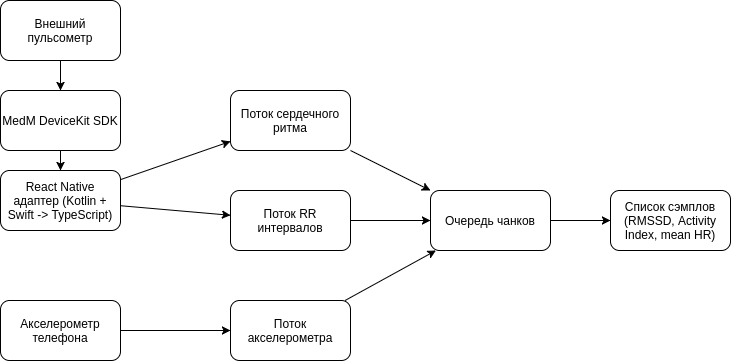
\includegraphics[width=\textwidth]{images/sensors_interaction.png}
  \caption{Взаимодействие с сенсорами}
  \label{fig:sensors_interaction}
\end{figure}

Необработанные данные представляют собой три потока из R-R интервалов,
сердечного ритма и показателей ускорения по трем осям мобильного телефона.
Данные из этих потоков записываются в соответствующие буферы, которые
периодически очищаются через фиксированный промежуток времени, а полученные
данные записываются в новый чанк (атомарный кусок данных, полученных с
сенсоров), который в свою очередь записывается в двустороннюю очередь
фиксированного размера. При поступлении нового чанка из очереди удаляется самый
старый чанк, а через фиксированный шаг в несколько чанков но основе данных,
содержащихся в очереди, считается новое измерение, которое также является
элементом выборки для модели машинного обучения. Такая архитектура сбора данных
позволяет разбить непрерывный поток данных на пересекающиеся отрезки
фиксированного размера и эффективно использовать память, храня только ту часть
данных, которая требуется для вычисления следующего измерения.

Перед подсчетом нового измерения данные сортируются по времени, т.к. вычисляемые
признаки зависят от их хронологии и существует вероятность, что порядок пакетов
данных полученных с пульсометра может быть нарушен из-за плохой связи с
сенсором. После сортировки вычисляются главные признаки: вариабельность
сердечного ритма, средний сердечный ритм и индекс физической активности. Далее
на основе вычисленных значений составляется вектор признаков для модели
машинного обучения.

\subsection{Взаимодействие с моделью}
Взаимодействие приложения с моделью машинного обучения заключается в сборе
обучающей выборки и последующей адаптации обученной модели для использования во
время выполнения приложения. Общая схема процесса обучения модели и его
взаимодействия показана на рис.~\ref{fig:model_interaction}.

\begin{figure}[ht]
  \centering 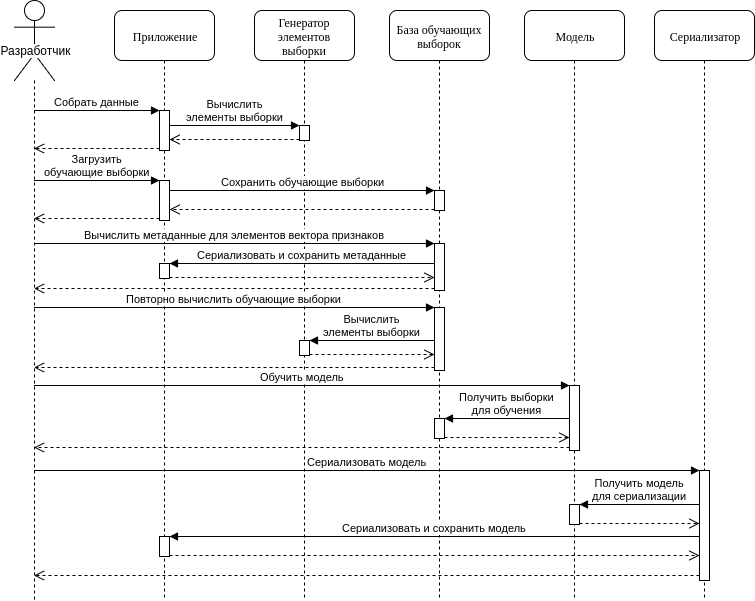
\includegraphics[width=\textwidth]{images/model_interaction.png}
  \caption{Взаимодействие с моделью}
  \label{fig:model_interaction}
\end{figure}

С целью упрощения работы с обучающей выборкой были написаны следующие скрипты:
``pull-samples'', ``calc-features-meta'', ``regenerate-samples'',
``train-model'' и ``serialize-model''. Чтобы понять, как они встраиваются в
процесс взаимодействия с моделью, нужно подробнее рассмотреть сам процесс.

Версия приложения для разработчика предусматривает возможность разметки
обучающей выборки и сохранения собранных данных в постоянном хранилище
мобильного телефона. Каждая попытка сбора данных порождает отдельную обучающую
выборку и сохраняет ее вместе с отметками и сырыми данными в отдельную
директорию, название которой является идентификатором выборки. После того, как
данные были собраны, с помощью скрипта ``pull-samples'' они загружаются на
машину, где будет проходить обучение модели.

Стоит заметить, что на этом этапе уже не требуется предварительная обработка
(включая стандартизацию) обучающей выборки, т.к. она была выполнена еще во время
сбора данных и реализована на TypeScript, чтобы не дублировать эту логику в
процессе обучения и непосредственного использования модели. Предварительная
обработка обучающей выборки состоит в составлении вектора признаков для каждого
элемента выборки. Он составляется на основе вычисленных показателей сердцебиения
и физической активности и базовых значений, полученных на этапе калибровки.

Далее модель обучается с помощью скрипта ``train-model'', передав ему
идентификаторы желаемых выборок, и сериализуется в JSON при помощи скрипта
``serialize-model'' для последующего использования в приложении. В самом
приложении во время выполнения используется не исходная модель, а ее
портированный аналог, который настраивается на основе сериализованных параметров
модели.

Перед подачей вектора признаков в модель он стандартизируется через
стандартизованную оценку (z-score), которая считается на основе стандартных
отклонений и средних значений элементов вектора. Эти значения вычисляются с
помощью скрипта ``calc-features-meta'', который также принимает на вход
идентификаторы выборок и сериализует полученные значения в JSON.

Отдельно стоит отметить скрипт ``regenerate-samples'', который пересчитывает
значения обучающих выборок на основе сохраненных сырых данных и базовых
значений. Он переиспользует всю логику вычисления обучающей выборки, благодаря
чему он крайне удобен в тех случаях, когда данные уже собраны, но выяснилось,
что для эффективной тренировки модели не хватает дополнительных признаков
или в вычислении признаков были ошибки (т.е. его можно использовать для
генерации обучающей выборки постфактум).

\section{Мобильное приложение}
\subsection{Интерфейс}
Интерфейс приложения состоит из трех основных и двух модальных экранов:

\begin{itemize}
\item Главный экран используется для приветствия, отображения прогресса сбора
  первичных данных, необходимых для отображения статистики, и самой статистики
  (рис.~\ref{screenshot:stats}). Последние значения главных показателей и
  состояния стресса находятся в верхней части экрана. При нажатии на значения
  показателей на графике отрисовывается его тенденция. Ползунок на графике можно
  использовать для просмотра статистики (главных показателей и продолжительности
  стресса) по прошедшему времени.
\item На экране настроек (рис.~\ref{screenshot:settings}) отображаются текущий
  сенсор, базовые значения сердцебиения и ошибка акселерометра. Также через него
  можно отсоединить текущий сенсор, сбросить значения калибровки и вызвать
  модальные окна (рис.~\ref{screenshot:sensors}) управления сенсорами и
  калибровки.
\item Экран разработчика (рис.~\ref{screenshot:dev}) содержит низкоуровневую
  статистику для отладки приложения и кнопки с уровнями стресса для разметки
  обучающей выборки.
\end{itemize}

\begin{figure}[ht]
  \begin{center}
    \subfigure[Экран статистики]{
      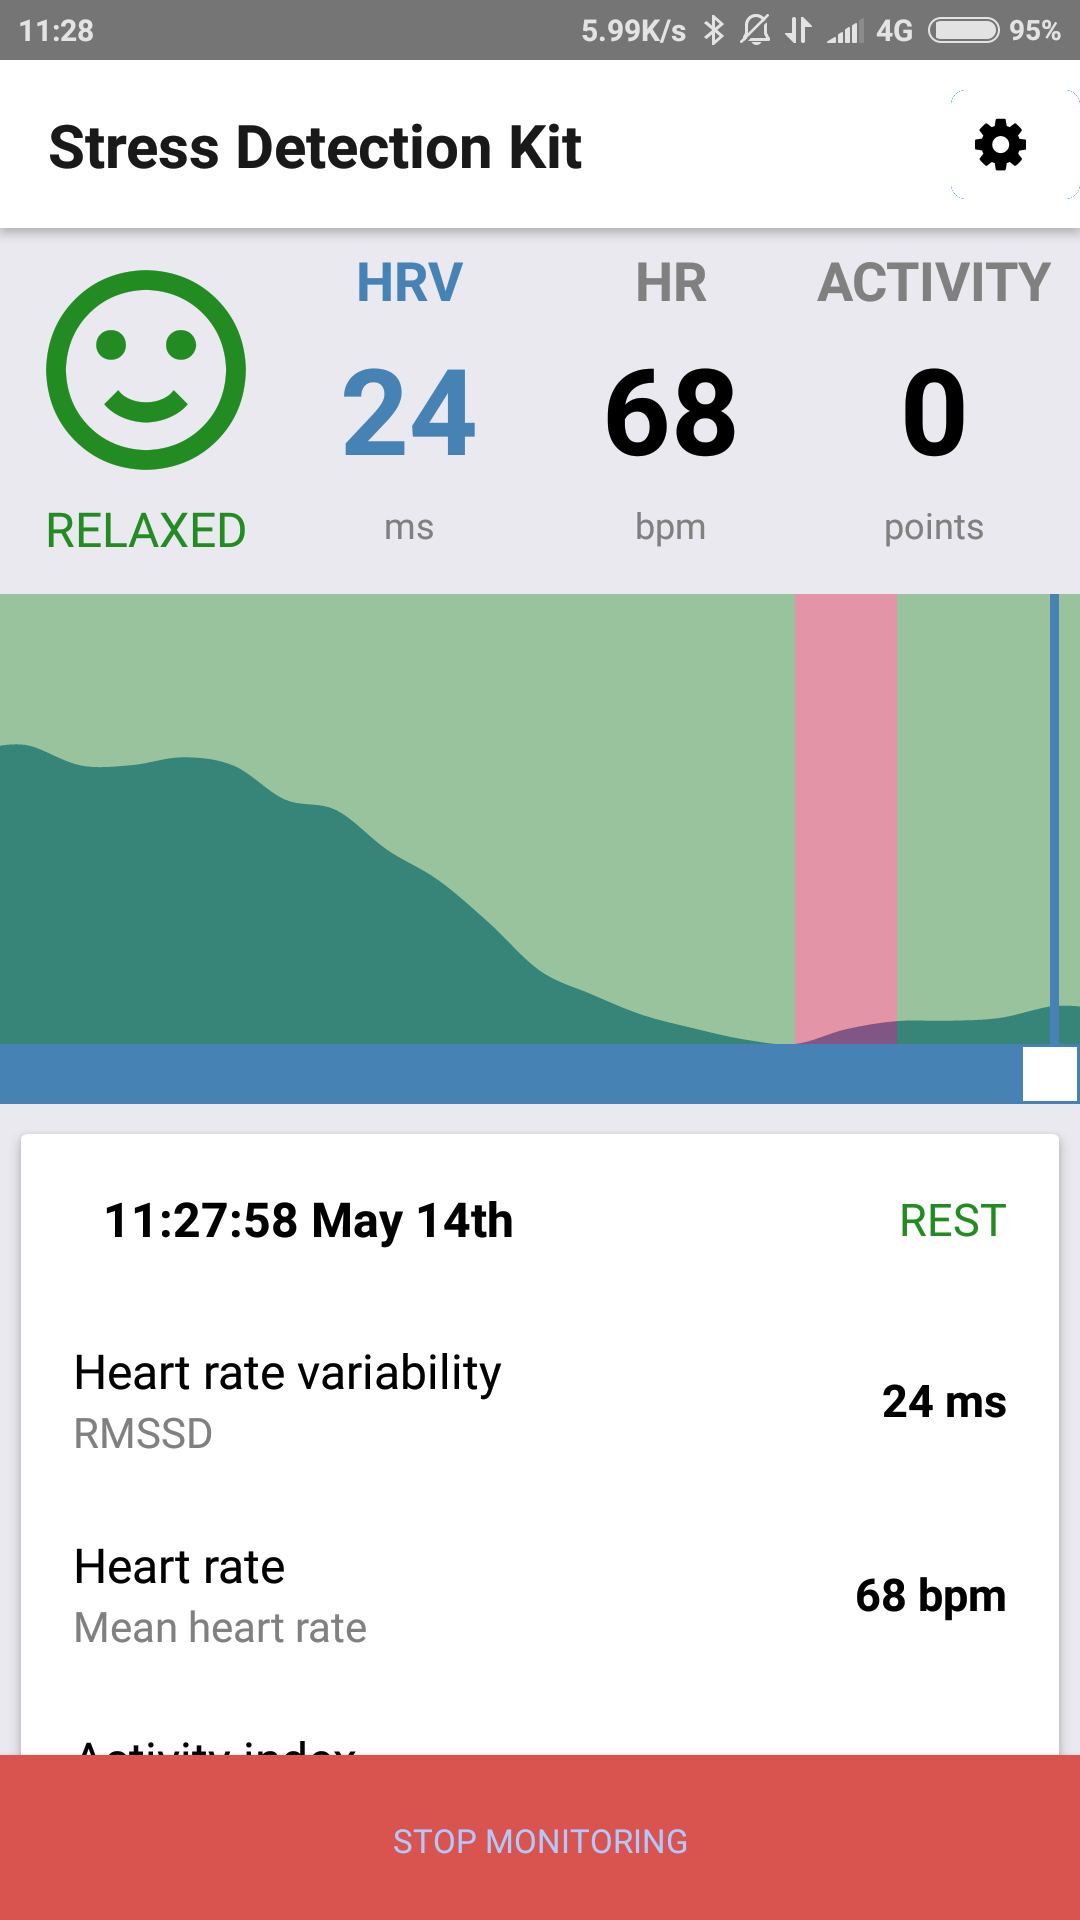
\includegraphics[width=0.4\textwidth]{images/stats_screen.png}
      \label{screenshot:stats}
    } \subfigure[Экран настроек]{
      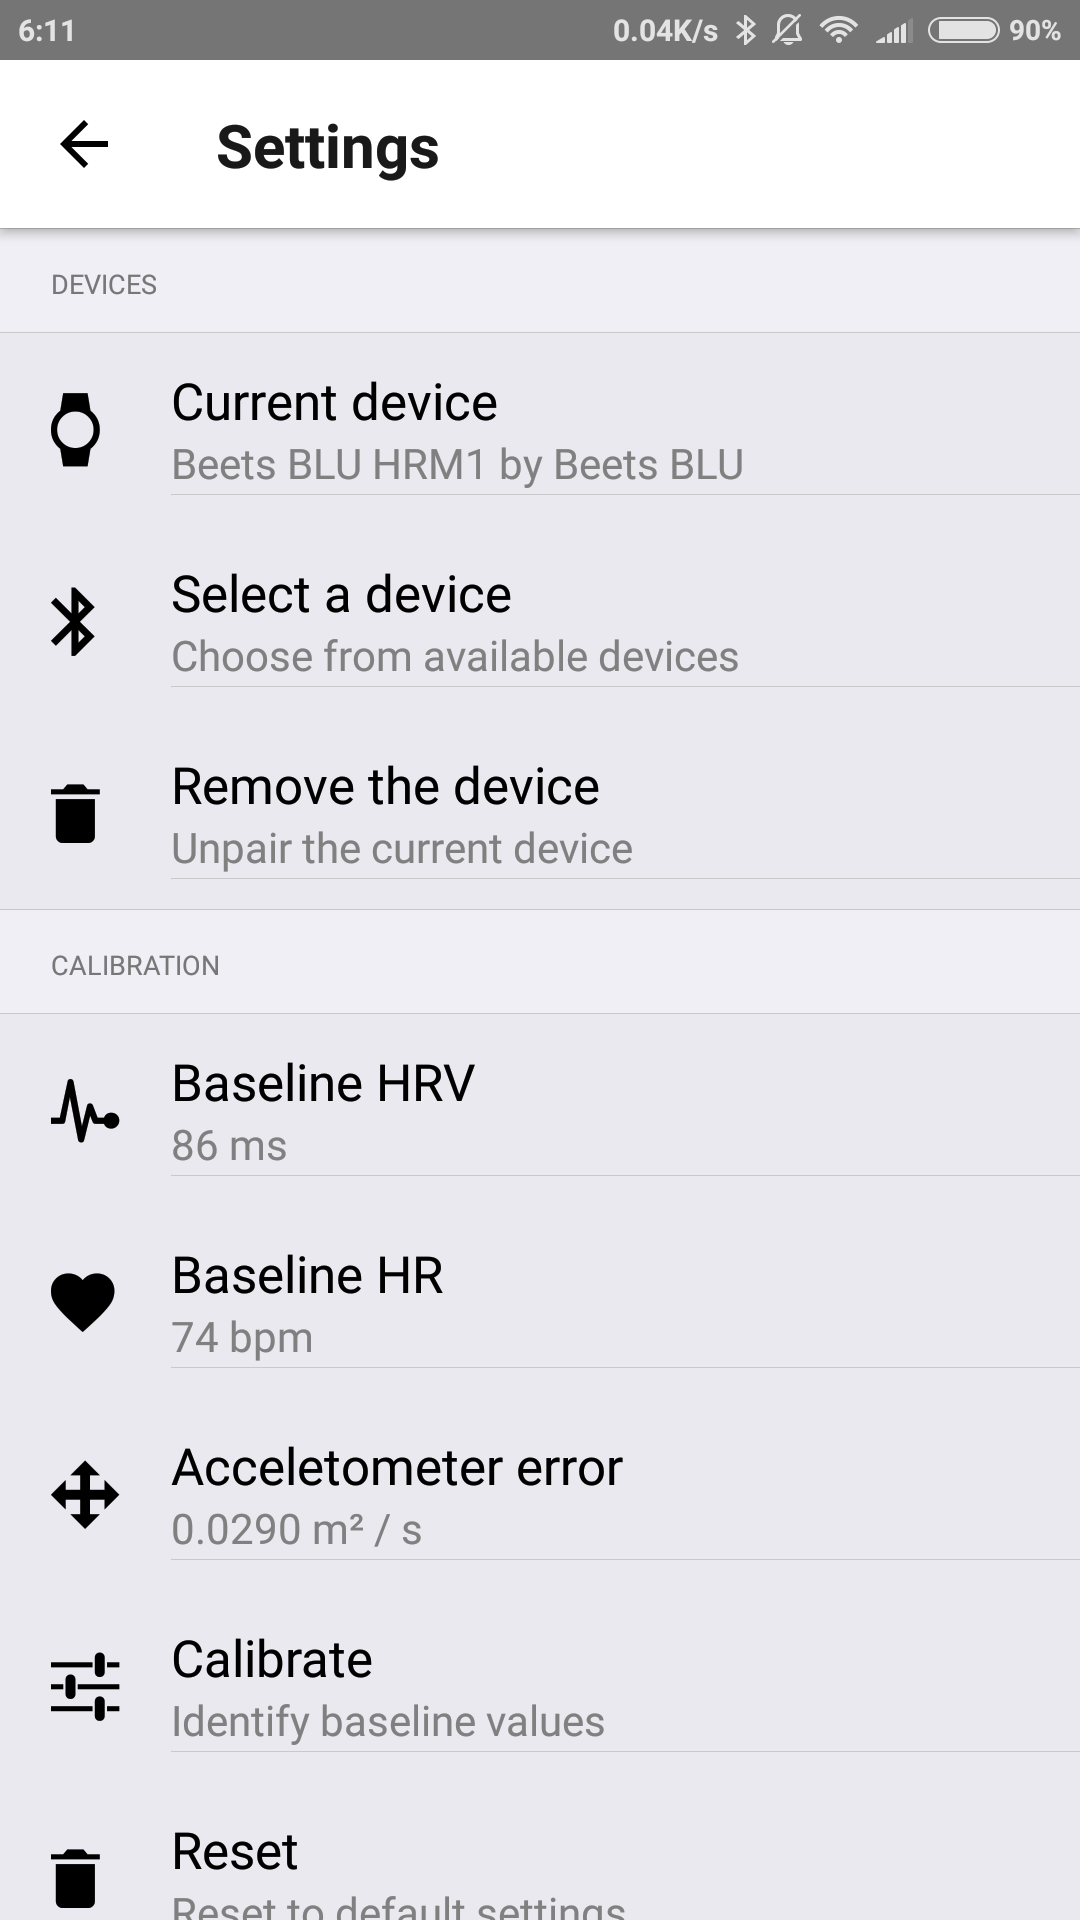
\includegraphics[width=0.4\textwidth]{images/settings_screen.png}
      \label{screenshot:settings}
    } \subfigure[Экран управления сенсорами]{
      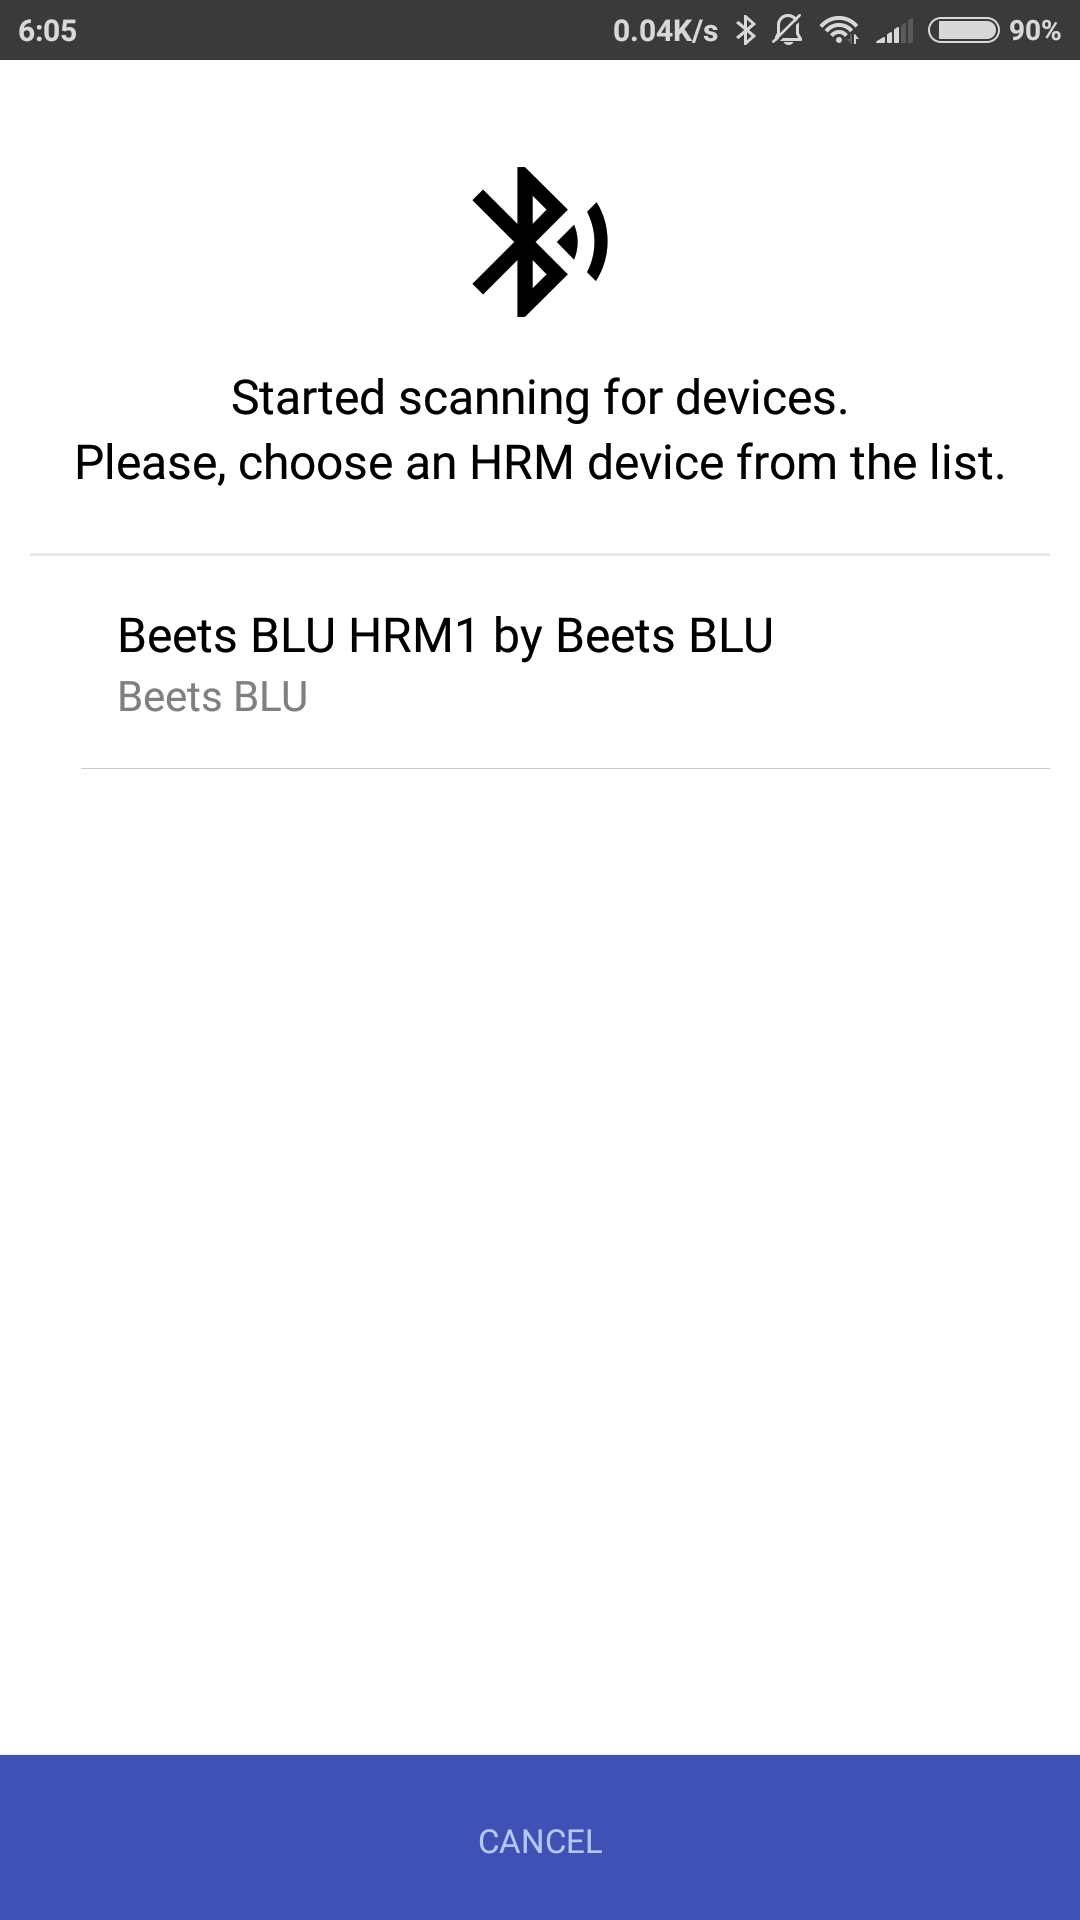
\includegraphics[width=0.4\textwidth]{images/sensors_screen.png}
      \label{screenshot:sensors}
    } \subfigure[Экран разработчика]{
      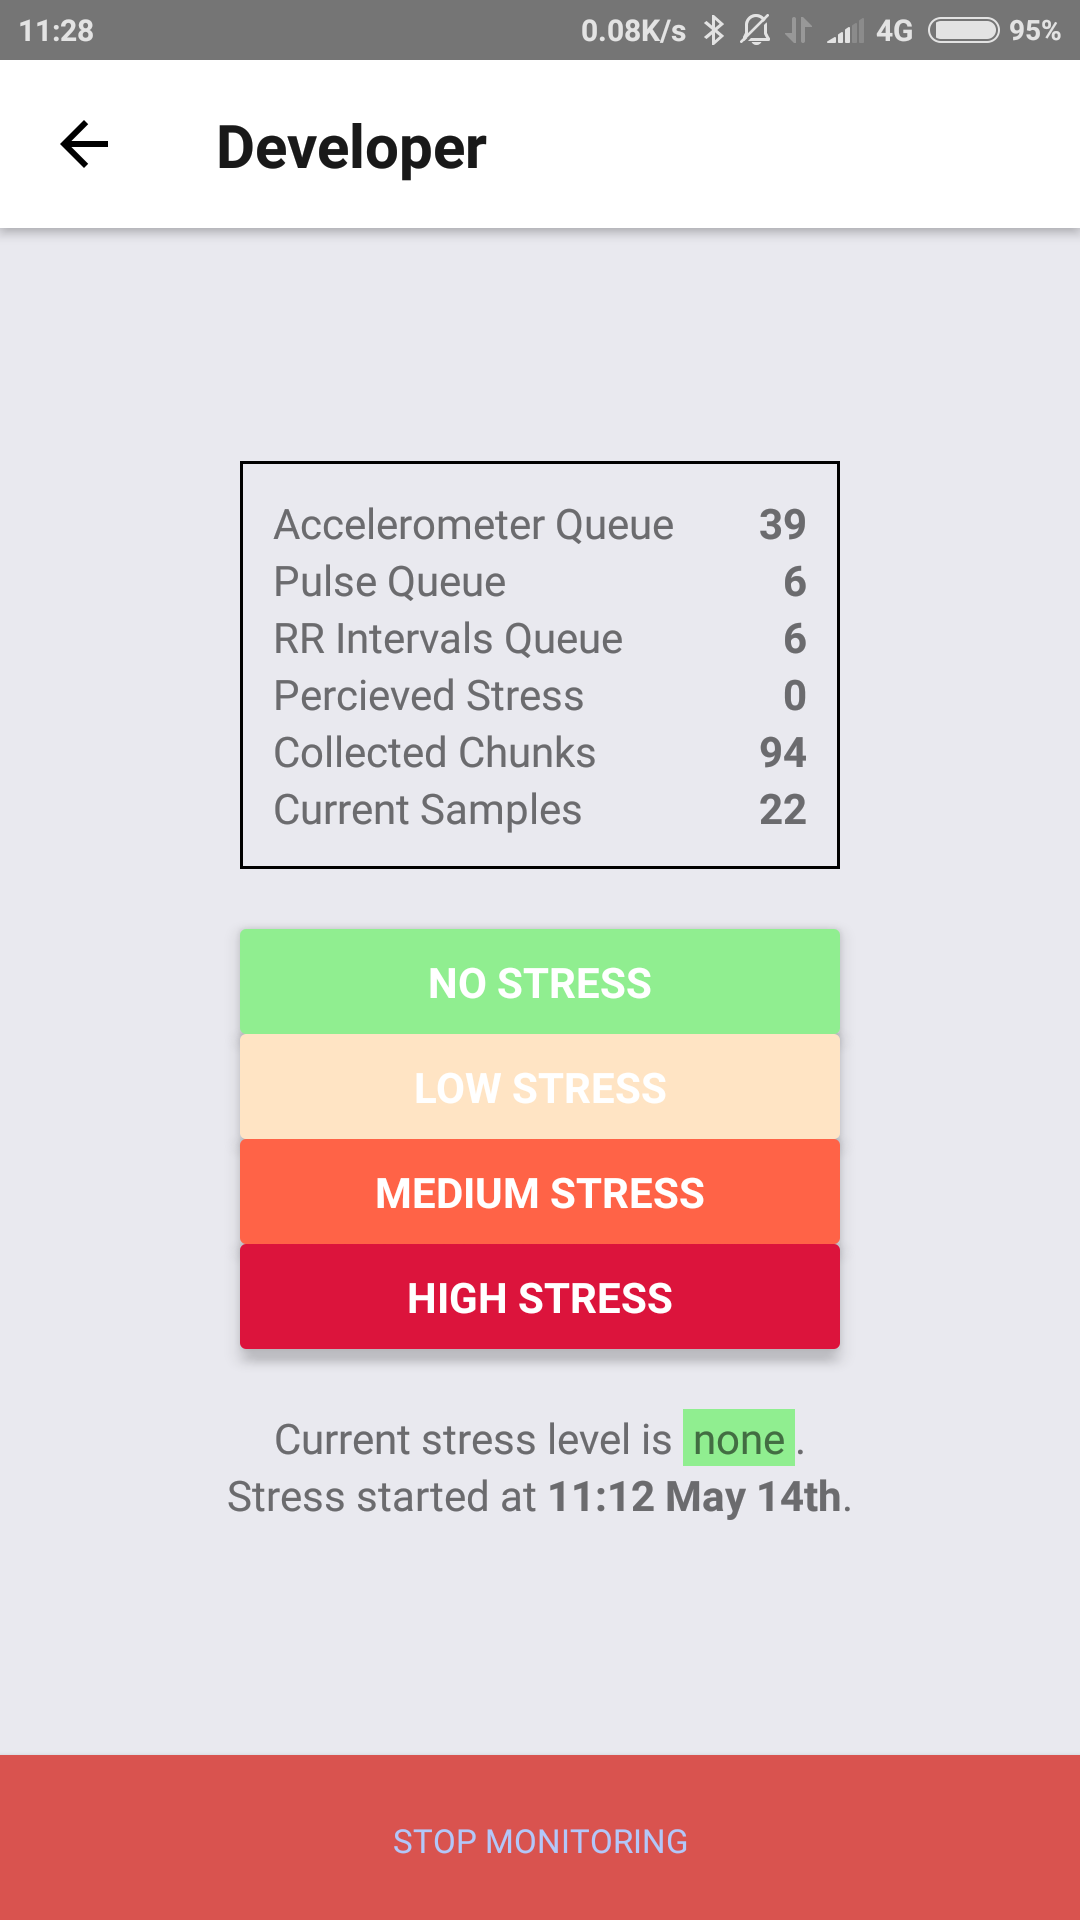
\includegraphics[width=0.4\textwidth]{images/dev_screen.png}
      \label{screenshot:dev}
    }
  \end{center}
	\caption{Экраны приложения}
	\label{screenshots}
\end{figure}

\subsection{Особенности реализации}
Несмотря на то, что экраны визуально не связаны между собой, они тесно связаны
на уровне данных. Например, главный экран и экран разработчика в реальном
времени показывают статистику, вычисленную по одним и тем же данным, а при
калибровке и подсчете статистики используются одни и те же механизмы (буферы
потоков и вычисление значений). Поэтому было принято решение разрабатывать
пользовательский интерфейс в реактивном стиле, что существенно упростило
разработку приложения.

Также для ускорения разработки была добавлена возможность сборки приложения с
ускоренным режимом (для этого нужно установить переменную среды
``ACCELERATED\_MODE''). В этом режиме нет необходимости подключать медицинский
сенсор, т.к. он заменяется генератором, который создает все данные
автоматически. В этом режиме промежуток времени между вычислениями нового
измерения сокращен до минимума, а этап сбора первичных данных вовсе отсутствует.

Версия приложения для разработчика, которая используется для сбора данных и
содержит экран разработчика, и версия для пользователя собираются из одной
кодовой базы в зависимости от выставленной переменной среды ``NODE\_ENV'',
которая может равняться значениям ``production'' и ``development''.

\section{Модель машинного обучения}
[Комментарий: эта часть работы еще не доделана, поэтому пока я описал только общий план.]

\subsection{Сбор данных}
The Trier social stress test (TSST).

Четыре уровня стресса при бинарной классификации.

\subsection{Выбор модели}
Классификация: SVM, RandomForest, Naive Bayes.

Без меток: K-means, OneClassSVM.

Сведение к регрессии по уровням стресса.

\subsection{Оценка эффективности}
Статистика по false positive и false negative в задаче классификации.

\section*{Заключение}
В рамках данной работы был создан прототип мобильного приложения для
автоматического отслеживания человеческого стресса в реальном времени. Показано,
что на основе данных с пульсометра и акселерометра можно эффективно определять
стресс в повседневной жизни. Более детально, были получены следующие результаты:

\begin{itemize}
\item Проанализированы существующие публикации на тему определения стресса на
  основе медицинских данных, выявлены недостатки в их подходах и выбраны
  наиболее важные показатели для определения стресса — вариабельность сердечного
  ритма и индекс физической активности.
\item Спроектирована архитектура приложения, позволяющая переиспользовать логику
  обработки данных с медицинских сенсоров во время выполнения и в процессе
  обучения модели, что в свою очередь помогает последовательно и независимо друг
  от друга разрабатывать мобильное приложение и модель машинного обучения.
\item Написано мобильное приложение для сбора данных с возможностью подключить
  пульсометр по bluetooth и отслеживать изменения в сердцебиении и физической
  активности на графике в реальном времени.
\item Собраны данные для обучения модели и на их основе обучена модель, которая
  была портирована в TypeScript, чтобы иметь возможность вызывать ее из кода
  приложения во время его выполнения, не отправляя данные во внешнюю систему.
\end{itemize}

\setmonofont[Path=assets/fonts/, UprightFont=*-Regular, BoldFont=*-Bold,
ItalicFont=*-Italic, BoldItalicFont=*-BoldItalic,
Mapping=tex-text]{CMUTypewriterText}

\bibliographystyle{assets/utf8gost705u} \bibliography{diploma}
\end{document}
